% !TEX root=/home/tavant/these/manuscript/src/manuscript.tex

\section{Presentation of the axial-azimuthal simulation}
\label{sec-ztheta_description}
The \ac{2D} simulation plane used so far in this work was the radial-azimuthal plane so that the plasma-wall interaction could be studied while obtaining self-consistently the azimuthal instability responsible for the axial electron transport.
In this configuration, we have implemented an algorithm that model the axial convection of the particles.
However, there are other missing mechanism of the axial direction in this simulation, in particular\string: the axial electric field is imposed\string; the wave is not convected\string; the impact of the axial gradients, such as the diamagnetic drift, are not included\string; the ionization region is not modeled.

The axial-azimuthal \ac{2D} simulation domain is used to study these mechanisms, and there are several studies that focused on modeling this specific simulation plane \citep{adam2004,coche2014,boeuf2018,taccogna2019}.
However, in these models, the impact of the radial direction is now missing.
Therefore, we propose in this chapter a first step to study the radial direction in the axial-azimuthal simulation.

After presenting the simulation domain and its characteristics in \cref{sec-ztheta_description}, we compare the impact of the radial losses modeled on the simulation results.
First, we analyze the discharge characteristics in \cref{sec-Zthetaresults}, then we focus in \cref{sec-Ztheta-instability} on the azimuthal instability.


\subsection{Description of the simulation domain} \label{subsec-ztheta_description}
To ease the understanding of the different simulation domains, \Cref{fig-3Dschematic} shows the simplified \ac{HET} annular channel with both the radial-azimuthal and the axial-azimuthal \ztheta domain.
The third \ac{2D} domain, the radial-axial domain, is not represented.
Indeed, it does not model the electron transport due to the azimuthal instability, hence we discard it.

\begin{figure}[hbt]
  \centering
  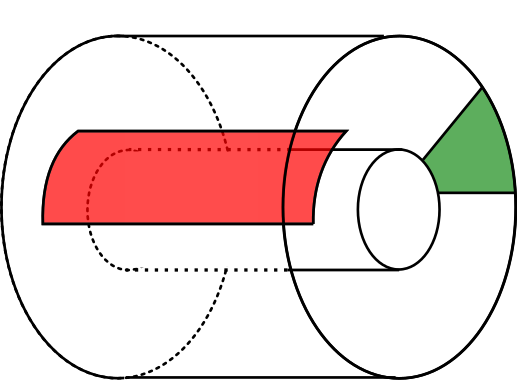
\includegraphics[width=0.5\textwidth]{3D_shematic}
  \caption{Schematic representation of the chamber of a \acs{HET} and (green) the radial-azimuthal and (red) the axial-azimuthal 2D domains.}
  \label{fig-3Dschematic}
\end{figure}

The \ac{2D} \ztheta domain is located at the mean radius of the channel\string; we neglect its curvature.
\Cref{fig-2D_ztheta_bis} presents a schematic representation of the \ztheta simulation domain.
The anode side is closed by a metallic fully absorbing electrode, with a fixed non-zero potential.
On the other side of the domain, the near-plume region (a few centimetres from the exit plane) is modeled.
The boundary located in the near-plume is also a Dirichlet boundary condition, this time grounded.
The azimuthal direction is closed with periodic boundaries for both the particles and the fields.

\begin{figure}[hbt]
  \centering
  \includegraphics[width=0.5\textwidth]{2D_ztheta}
  \caption{Schematic representation of the \acs{2D} \ztheta simulation domain.}
  \label{fig-2D_ztheta_bis}
\end{figure}

The axial and azimuthal electric fields are self-consistently computed from the charge density by solving the Poisson equation.
Consequently, the simulation domain is not so different from the radial-azimuthal simulation domain.
This allowed us to adapt the code \LPPic to simulate both domains using the same core functions.
Three particular aspects have been developed\string: the cathode electron emission, the dynamic computational load balancing, and the electron sub-cycling.

\paragraph{Cathode electron emission\\}
In the \ac{HET},  the cathode is are mostly used to neutralize the ion beam, but a significant fraction of the emitted elections enters the channel and travels toward the anode, maintaining the discharge.
Consequently in the simulation, electrons are injected close to the cathode boundary following a Maxwellian distribution of a few electron volts.
The number of electrons to inject at each time step is computed by closing the eternal circuit between the anode and the cathode.

In the experimental set-up, an electric filter is placed between the thruster and the generator \citep{barral2008}, originally placed to protect the power supply against AC current.
While this external circuit can be modeled \citep{verboncoeur1993}, and is susceptible to impact the thruster behavior \citep{barral2008,wei2017}, we neglect it in this study for sake of clarity.
Thus, the cathode current equals the anode current \[ I_a = I_c. \]

\paragraph{Dynamic computational load balancing\\}
The axial profile of the plasma density presents a maximum that can be one order of magnitude higher than the mean plasma density.
Consequently, a static MPI domain decomposition would produce an unbalance in the number of numerical particles per CPU, which would result in an under-efficient code.

One possibility is to modify dynamically the weight of the numerical particles relative to the plasma density, in order to keep a relatively constant number of particles per cell.
This can be done by merging the particles when they are too small, or by splitting them in smaller particles when they are too big \citep{shon2001,teunissen2014}.
However, such algorithm can modify the charge, momentum, or the energy of the system if not done carefully.
In \citet{vranic2015}, the authors present an algorithm claimed to conserve these quantities.
However, we chose not to implement it because of its error-prone complexity.

Instead, we implemented a dynamic redistribution of the CPU domain, so that every CPU own approximately the same number of particles.
As the density gradient is principally in the axial direction, we only change the axial size of the CPU domains.

\paragraph{Electron time-step sub-cycling\\}
Due to the large mass ratio between the  ions and the electrons, the ion dynamic is much slower than the electron dynamic that constrained the time step  $\dt$, which is constrained by the electron dynamic.
In \citet{adam1982}, the authors propose to reduce the computational time by using a different time-step $\dt$ for the ions and the electrons.
They show theoretically and numerically that numerical instabilities rise when $\ope \dt_i  \sim \pi$.
With the stability criterion on $\dt_e$ \cref{eq-dx_limit}, we find the stability criterion 
\begin{equation} \label{eq-subcycling_criterion}
  \frac{\dt_i}{\dt_e} < \frac{\pi}{0.2} \simeq 15.7.
\end{equation}

Consequently, we use $\frac{\dt_i}{\dt_e} = 11$ in the latter.
We verified for one case that using the same time-step for the ion and the electrons produces the same solution.


\subsection{Facing the breathing mode} \label{subsec-breathmod}
The breathing mode comes from the coupling between the neutral gas flow and the plasma dynamics, via the ionization.
Under the typical conditions of the \ac{HET}, we observed this oscillation with a low frequency, around  $10-30$ kHz, and a large amplitude, as the plasma density can change up to one order of magnitude during the oscillation period \citep{barral2003a,barral2009}.
This oscillation is much slower than the \ac{ECDI}, and is present throughout the entire channel.

If these oscillations are not problematic for the fluid or \ac{DK} simulations, they are for \ac{PIC} simulations.
Indeed, the total number of numerical particles is proportional to the plasma density, and a minimal number of particles is required to limit the numerical heating \citep{turner2006}.
Thus, when the mean plasma density oscillates, the number of numerical particles (hence the amount of memory used) can change drastically.
This reduces significantly the performance of the simulation code, and can lead to memory overflow if the memory available is not high enough to store all of the particles during the peak of density  of the oscillation.
The \emph{merging-splitting} of the particles  can be used to reduce the variation of the number of numerical particles, but it is not used for the same reason than discussed above.

In addition to the number of particles, the numerical parameters (time step and cell size) have to be chosen to satisfy the stability criteria during all of the simulation, which also reduces significantly the performance of the simulation. 
This could be overcome by adapting dynamically the mesh and the time step.
However, too few studies of the consequences of the use of adaptive mesh and time step on the simulations have been conducted.
Thus, we have chosen not to modify the \ac{PIC} algorithm.

Two other approaches have been followed to reduce the computational cost induce by the breathing mode\string:
\begin{enumerate}
  \item the approach used by \citet{coche2014}\string: using a scaling of the permittivity to reduce the computational load,
  \item the approach of \citet{boeuf2018}, using a forced ionization source term.
\end{enumerate} 
These two cases are significantly different in the physics modeled and the behavior observed, as Boeuf's test-case will converge toward a steady-state, in contrast to Coche's test-case which model the breathing mode.
Since we are not directly interested in the breathing oscillations, we use in this study the test-case of Boeuf.

% 
% \subsection{Simulation test-case of Coche} \label{subsec-coche_description}
% 
%   The simulation proposed by \citet{coche2014} models self-consistently the ionization with the \ac{MCC} algorithm, as well as the neutral gas flow.
%   \Cref{fig-coche-presnetation} presents the domain of simulation.
%   The simulation domain geometry is realistic, with a channel length $L_{channel} = 2.5\,\centi\meter$ for a total axial length of the simulation domain $L_z=4\,\centi\meter$.
%   Hence, the totality of the chamber and a part of the near plume is simulated.
% 
%    \renewcommand\subfigurewidth{0.48\textwidth}
% 
% 
%   \begin{figure}[hbt]
%     \centering
%     \begin{tabular}{@{} cc}
%       \subfigure{coches_domain}{}{10,10} &
%       \subfigure{coches_profiles}{}{10,10} \\
%     \end{tabular}
%     \caption{(left) the \acs{2D} axial azimuthal domain; (right) the axial profile of the magnetic field and the initial xenon neutral gas profile used for the simulation case of Coche. }
%     \label{fig-coche-presnetation}
%   \end{figure}
% 
% 
%   The neutral xenon is modeled by solving a system of \ac{1D} fluid equations.
%   Indeed, the azimuthal variations of the neutrals are neglected in this section.
%   The gas is modeled using the continuity and the momentum conservation equations\string:
%   \begin{align}
%     \deriv{n_g}{t} &+ \deriv{(n_g v_g)}{z} = - S_{iz} \\
%     \deriv{(n_g v_g)}{t} &+ \deriv{(n_g v_g^2)}{z} +  2 \deriv{( n_g D_g)}{z} = - S_{iz} v_g
%   \end{align}
% 
%   with $n_g$ and $v_g$ the neutral gas density and axial velocity, respectively, $S_{iz}$ is the ionization source term obtained by the \ac{MCC} algorithm, and $D_n$ is used to close the system, and is \citep{coche2013}
%   \begin{equation} \label{eq-Dn}
%     D_n = \frac{k_B T_g}{6 m_i}.
%   \end{equation}
%   The gas temperature $T_g=640K$ and the initial condition is described on the density $n_g$ on \cref{fig-coche-presnetation}(right).
%   The initial velocity is $v_g=200\,\meter\per\second$.
% 
% 
%   The constraints on the time step and the cell size are alleviated by using a scaling on the permittivity.
%   It is simply increased by a coefficient $\alpha$, as used in other low-temperature modelling \citep{fubiani2012,boeuf2012,liu2010}.
%   The electron plasma frequency and electron Debye length thus become (starred quantities)
%   \begin{equation} \label{eq-scaled_lde}
%     \lde^* = \sqrt{\frac{\alpha \epsilon_0 \Te}{e n_e}} = \lde \alpha^{1/2}
%   \end{equation}
%   \begin{equation} \label{eq-scaled_wpe}
%     \ope^* = \sqrt{\frac{e^2 n_e}{\alpha \epsilon_0 m_e}} = \ope \alpha^{-1/2}
%   \end{equation}
%   Hence, the constraints on the time step and the cell size are reduced by a factor $\sqrt{\alpha}$
%   \begin{align*}
%     \Delta t ^* &= \alpha^{1/2} \Delta t \\
%     \Delta x ^*&= \alpha^{1/2} \Delta x  
%   \end{align*}
% 
%   By using a factor $\alpha=80$,  which correspond to a factor of $9$ on the time step and the cell size,  \citet{coche2014} successfully observed the breathing mode in the \ac{PIC}-\ac{MCC} simulation.
%   The physical and numerical conditions used for the test-case of Coche are given in \cref{tab-parameters-coche}.
% 
%   The cathode emitted electrons are injected at the boundary, using a Maxwellian flux distribution.
%   The plume neutralization is not described, thus the current to inject is
%   \begin{equation} \label{eq-coche_Ice}
%     I_{ce } = I_a + I_b
%   \end{equation}
%   with $I_a$ the total current collected at the anode boundary $I_a = I_{, i} + I_{a, e}$ and $I_b$ the beam current $I_{b} = I_{b, i} + I_{b, e}$. 
%   At the anode, the current is mostly composed of the electron current, while the beam is mostly composed of ions.
% 
%   \begin{table}[htb] %PIC parameters
%        \centering
%        \ra{1.3}
%        \caption{\label{tab-parameters-coche} Physical and numerical parameters used in the \acs{2D} \acs{PIC} simulations of an axial and azimuthal \ztheta plane of a \acs{HET} in the test-case of Coche.}
%        \begin{tabular}{@{}r c c c@{}} 
%           \toprule
%           {\bf Physical Parameter} & notation & Value & Unit \\
%           \midrule
%           Gas & & Xenon & - \\
%           Domain dimensions & $L_{\theta} \times L_{z}$ & $4.6 \times 4.0$ & [cm$^2$] \\
%           Maximum magnetic field & $\max(B_{r})$                    & $170$                 & [{G}] \\
%           Position of  $\max(B_{r})$   & $z_{\max(B_{r})}$                    & $2.5$      & [cm] \\
%           Anode voltage & $U_d$                    & $300$     & [V] \\
% 
%           Initial electron temperature & $\Te_{,0}  $               & $1.0$                 & [{V}] \\
%           Initial ion temperature & $T_{i,0}   $               & $1.0$                 & [{V}] \\
%           Neutral gas pressure & $P_{n}     $               & $2.0$                 & [{mTorr}] \\
%           Neutral gas temperature & $T_{n}     $               & $640$                 & [{K}] \\
%           Neutral gas density & $n_{g}     $               & $3.0 \times 10^{19}$ & [{m}$^{-3}$]\\
%           Initial plasma density & $n_0$ & $\sn{1}{18}$ &  [{m}$^{-3}$]\\
%           \midrule
%           {\bf Simulation Parameter} &  &   &  \\
%           Permittivity scaling & $\alpha$ & 80 & - \\
%           Cell size & $\Delta x = \Delta y$ & $3.6 \times 10^{-4}$  & [{m}] \\
%           Time step & $\Delta t  $                      & $2.7 \times 10^{-11}$ & [{s}] \\
%           Electron sub-cycling & $\frac{\dt_{i}}{\dt}$ & 11 & - \\
%           Initial number of particles per cell & $N/NG      $    & $200$   & [{part/cell}] \\
%           \bottomrule
%        \end{tabular}
%     \end{table}
    
\subsection{Description of the simulation test-case of Boeuf} \label{subsec-boeuf_description}

In \citet{boeuf2018}, the authors used a simplified simulation set-up in order to study the azimuthal instabilities.
The simulation is collisionless and the ionization profile is not-self-consistent but is rather given as an input.
This removes the breathing mode oscillations from the discharge, and simplifies the parametric study.
The ionization source term $S_{iz}$ used follow a cosine profile
\begin{equation} \label{eq-siz_profile}
  S_{iz} = \max \lp 0, S_0 \cos \left[ \pi \frac{z - z_M}{L_S} \right] \rp,
\end{equation}
with the parameters $S_0, z_M$ , and $L_S$ given in \cref{tab-parameters-boeuf}.
The simulation domain is small, reducing again the computational load.
Indeed, the axial length in this case in $L_z=2.5\,\centi\meter$, with $L_{ch}=0.75\,\centi\meter$ of the chamber included in the simulation domain, against $L_{ch}=2.5\,\centi\meter$ in the typical \ac{HET}.
\Cref{fig-boeuf-presnetation} presents the simulation domain and the axial profile of the ionization source term $S_{iz}$ and the magnetic field.
\begin{figure}[hbt]
  \centering
  \begin{tabular}{@{} cc}
    \subfigure{boeuf-domain.png}{}{10,10} &
    \subfigure{boeuf-profiles.png}{}{10,10} \\
  \end{tabular}
  \caption{(left) the \acs{2D} axial azimuthal domain\string; (right) the axial profile of the magnetic field and the ionization source term profiles used for the simulation case of Boeuf. }
  \label{fig-boeuf-presnetation}
\end{figure}

The electrons emitted by the cathode are injected inside of the simulation domain, at 1\,cm from the boundary.
Since the electron injection is not located at the cathode boundary, a large cathode sheath is present.
Therefore, the plasma potential is corrected so that the potential is $\phi=0$ at the location of injection, at 1\,cm from the boundary.
This is done by substracting the azimuthally averaged plasma potential at the injection plane, from the potential calculated with the Poisson equation.
The physical and numerical conditions used for the test-case of Boeuf are given in \cref{tab-parameters-boeuf}.

\begin{table}[htb] %PIC parameters
     \centering
     \ra{1.3}
     \caption{\label{tab-parameters-boeuf} Physical and numerical parameters used in the \acs{2D} \acs{PIC} simulations of an axial and azimuthal \ztheta plane of a \acs{HET} in the test-case of Boeuf.}
     \begin{tabular}{@{}r c c c@{}} 
        \toprule
        {\bf Physical Parameter} & notation & Value & Unit \\
        \midrule
        Gas & & Xenon & - \\
        Domain dimensions & $L_{\theta} \times L_{z}$ & $1.25 \times 2.5$ & [cm$^2$] \\
        Maximum magnetic field & $\max(B_{r})$                    & $100$                 & [{G}] \\
        Position of  $\max(B_{r})$   & $z_{\max(B_{r})}$                    & $0.75$      & [cm] \\
        Anode voltage & $U_d$                    & $200$     & [V] \\
        Initial electron temperature & $\Te_{,0}  $               & $10.0$                 & [{V}] \\
        Initial ion temperature & $T_{i,0}   $               & $0.5$                 & [{V}] \\
        Initial plasma density & $n_0$ & $\sn{5}{16}$ &  [{m}$^{-3}$]\\
        Maximum Ionisation & $S_0$ & $\sn{5.23}{23}$  & [{m}$^{-3}${s}$^{-1}$]\\
        Center of $S_{iz}$ profile & $z_M$ & $0.625$  & [{cm}]\\
        Width of $S_{iz}$ profile & $L_S$ & $0.75$  & [{cm}]\\
        \midrule
        {\bf Simulation Parameter} &  &   &  \\
        Permittivity scaling & $\alpha$ & 1 & - \\
        Cell size & $\Delta x = \Delta y$ & $5 \times 10^{-5}$  & [{m}] \\
        Time step & $\Delta t  $                      & $5 \times 10^{-12}$ & [{s}] \\
        Electron sub-cycling & $\frac{\dt_{i}}{\dt}$ & 11 & - \\
        Initial number of particles per cell & $N/NG      $    & $25$   & [{part/cell}] \\
        \bottomrule
     \end{tabular}
  \end{table}



\subsection{Model for radial losses} \label{subsec-fakeR}

In this section, we address the objective to add to the purely \ac{2D} axial-azimuthal \ac{PIC} simulation the impact of the radial walls.
The first effect that we want to model is the particle and power losses to the wall.
Thus, as previously done in the radial-azimuthal simulation, the particles are tracked in the three directions, and a finite radial length is used to limit the radial direction.

When an ion crosses the boundary, it is removed from the simulation.
The electrons are partially reflected, such that the electron flux absorbed at the wall equals the ion flux.
We do not model the secondary electron emission.
We suppose that the sheath is infinitely thin, so that the wall corresponds to a partially reflecting surface.
Two approaches have been investigated to model efficiently the effect of the sheath.


\paragraph{ Model 1 for the radial losses\string: sheath model\\}
In the first approach, we set the potential drop at the walls by the use of a sheath model, such as the one described in \cref{sec-sheath}, or in \cref{ch-3,ch-4}.
The ions would be absorbed by the radial boundary, as well as the electrons of energy higher than the sheath potential.
Electrons with smaller energy are reflected spectacularly.

This model is more physical, and it would allow local charge imbalance.
However, as there is no electric field self-consistently computed in the radial direction, the plasma cannot react to such imbalances.
Hence, we chose not to use it.

% \paragraph{ Model 2 for the radial losses\string: fixed sheath potential\\}
% In \citet{coche2014}, the authors simulate the electron-wall collisions we setting a sheath potential of $20\,\volt$.
% Electrons, whose energy directed along the radial direction is larger than the value of sheath potential, are likely to undergo wall collisions.
% For each of these electrons, the authors calculate a collision frequency that can be roughly estimated by $\nu_{ew} = 1⁄4 v_r/L_R$, where $v_r$ is the electron velocity in the radial direction and $L_R$ is the channel width.
% If the collision occurs, the electron is isotropically reflected and does not suffer from any energy losses.
% The authors did not modeled the particle losses

\paragraph{Model 2 for the  radial losses\string: flux equality\\}
The second approach directly imposes the flux equality by absorbing every time step the same number of electrons than ions.
The electrons crossing the radial boundaries are sorted by their energy in the radial direction, and the electrons absorbed are the most energetic ones.
The others are reflected elastically.
Due to the small number of ions crossing the boundary, and for performance issues, we choose to impose the flux equality averaged over the domain of a CPU.
As 360 CPU domains are used to decompose the whole simulation domain, this allows a partial locality of the flux equality. 

\vspace{1ex}
While the sheath can be supposed infinitely thin, the ion flux to the wall usually depends on the pre-sheaths, which display an ambipolar electric field that accelerates the ions to the ion sound speed at the sheath edge.
Since the development and validation of a pre-sheath electric field model in the radial model required more resources than available, there is no such pre-sheath model in the results presented in this chapter.
Consequently, the ion flux to the wall is a thermal flux, which is much smaller than the flux created by a pre-sheath.
Hence, using a realistic radial length  of the order of $2\,\centi\meter$, the particle losses are underestimated.
One solution could be to reduce the radial length, so that the particle flux are closer to physical losses.

The results given in the next sections are obtained by modeling the radial losses in the whole simulation domain.
We choose to do so in order not to introduce a discontinuity in the radial boundary condition, as well as to increase the impact of the radial losses on the simulation results.
